%%%%%%%% ICML 2026 PREPRINT LATEX SUBMISSION FILE %%%%%%%%%%%%%%%%%

\documentclass{article}

\usepackage{microtype}
\usepackage{graphicx}
\usepackage{subcaption}
\usepackage{booktabs}
\usepackage{multirow}
\usepackage{adjustbox}
\usepackage{amsmath}
\usepackage{amssymb}
\usepackage{mathtools}
\usepackage{amsthm}
\usepackage[capitalize,noabbrev]{cleveref}
\usepackage{xcolor}
\usepackage{enumitem}
\usepackage{algorithm}
\usepackage{algorithmic}
\usepackage{tikz}
\usetikzlibrary{arrows.meta,positioning,shapes.geometric,fit,calc}

\usepackage[preprint]{icml2026}

\newcommand{\ours}{\texttt{RLS}}
\newcommand{\systemname}{\texttt{Reflective Loop Skills}}
\newcommand{\roadmap}{\texttt{roadmap.md}}
\newcommand{\activestate}{\texttt{active\_task.json}}
\newcommand{\failurebank}{\texttt{failure\_bank.json}}
\newcommand{\lastmode}{\texttt{last\_mode.txt}}

\definecolor{rlblue}{RGB}{38,113,191}
\definecolor{rlgreen}{RGB}{42,143,91}
\definecolor{rlorange}{RGB}{219,132,45}
\definecolor{rllight}{RGB}{246,248,252}

\newcommand{\theHalgorithm}{\arabic{algorithm}}

\theoremstyle{plain}
\newtheorem{theorem}{Theorem}[section]
\newtheorem{proposition}[theorem]{Proposition}
\newtheorem{lemma}[theorem]{Lemma}
\newtheorem{corollary}[theorem]{Corollary}
\theoremstyle{definition}
\newtheorem{definition}[theorem]{Definition}
\newtheorem{assumption}[theorem]{Assumption}
\theoremstyle{remark}
\newtheorem{remark}[theorem]{Remark}

\icmltitlerunning{Reflective Roadmaps Are Weights}

\begin{document}

\twocolumn[
\icmltitle{Reflective Roadmaps Are Weights: A Training View of Long-Horizon Agent Loops}

\begin{icmlauthorlist}
  \icmlauthor{Anonymous Authors}{anon}
\end{icmlauthorlist}
\icmlaffiliation{anon}{Anonymous Institution}
\icmlcorrespondingauthor{Anonymous Authors}{anonymous@example.com}
\icmlkeywords{LLM agents, coding agents, self-improvement, agent memory, multi-agent orchestration}
\vskip 0.3in
]

\printAffiliationsAndNotice{}

\begin{abstract}
Long-horizon agents fail less like weak reasoners than like systems without durable training state: they forget the objective, repeat local repairs, and restart from brittle transcripts after every interruption. We argue that the missing object is the roadmap. In a persistent agent loop, the roadmap plays the role of weights: a slow, reusable carrier of task structure against which fast local adaptation should be performed. We formalize this view through \systemname{} (\ours), a non-parametric training loop for coding agents in which the roadmap is the backbone, \activestate{} is the adapter, check results are loss signals, local patches are update directions, and \failurebank{} is error memory. This framing turns ``looping'' from a scheduling trick into an optimization interface for long tasks. We instantiate the interface across seven CLI agents and extend it with \texttt{moa-loop}, where a single vertical loop becomes a mixture-of-agents computation graph with DAG scheduling and shared blackboard communication. We further separate trigger mechanisms---Stop hooks, external daemons, OS-level cron schedulers with differential health-check intervals, and application-level schedulers---from the persistent state contract they must preserve. The contribution is a training-centric architecture for agents that continue, correct, and accumulate work across epochs without updating neural weights.
\end{abstract}

\section{Introduction}

Large language model (LLM) agents have become increasingly capable at tool use, code editing, and autonomous problem solving \citep{codeact,alphaevolve,automind}. In software engineering settings, they can inspect repositories, synthesize patches, run tests, and revise their own outputs. Yet the task regime that motivated this work is not the short edit; it is the long task. Long tasks require the agent to keep moving after interruptions, partial failures, context loss, and repeated verification cycles. The dominant interaction pattern remains surprisingly short-lived: a user opens a session, the agent reasons through the current task, local feedback is consumed in the moment, and much of the operational knowledge disappears when the session ends.

Experience-driven agents and procedural memories address parts of this problem by storing trajectories, reflections, workflows, or skills \citep{expel,voyager,awm,memp,legomem,xu2025amemagenticmemoryllm}. These approaches highlight a common insight: capable agents should not rediscover the same behavior every time. Our work arrived at a stronger systems claim: for long tasks, the roadmap becomes as important as the model prompt itself. It is the slow state that preserves what the project is trying to become. Raw transcripts are too noisy for this role, while a single prompt is too brittle to represent both global strategy and local adaptation.

We introduce \systemname{} (\ours), a repository-level pattern for persistent, self-correcting coding agents. \ours{} is implemented as seven loop skills targeting common agent CLIs: Codex, Gemini, Claude, Qwen, Kimi, MiniMax, and Cursor, plus \texttt{moa-loop} for multi-agent orchestration. Each skill follows the same reflective loop: an optimize pass performs a bounded slice of work, a check pass audits the result, the check pass writes local patches, and the next epoch conditions on those patches. The design deliberately mirrors the deep-learning recipe at the orchestration level. The roadmap is the slow backbone, \activestate{} is the fast adapter, check findings are loss signals, and local patches are externalized update directions.

\begin{figure*}[t]
\centering
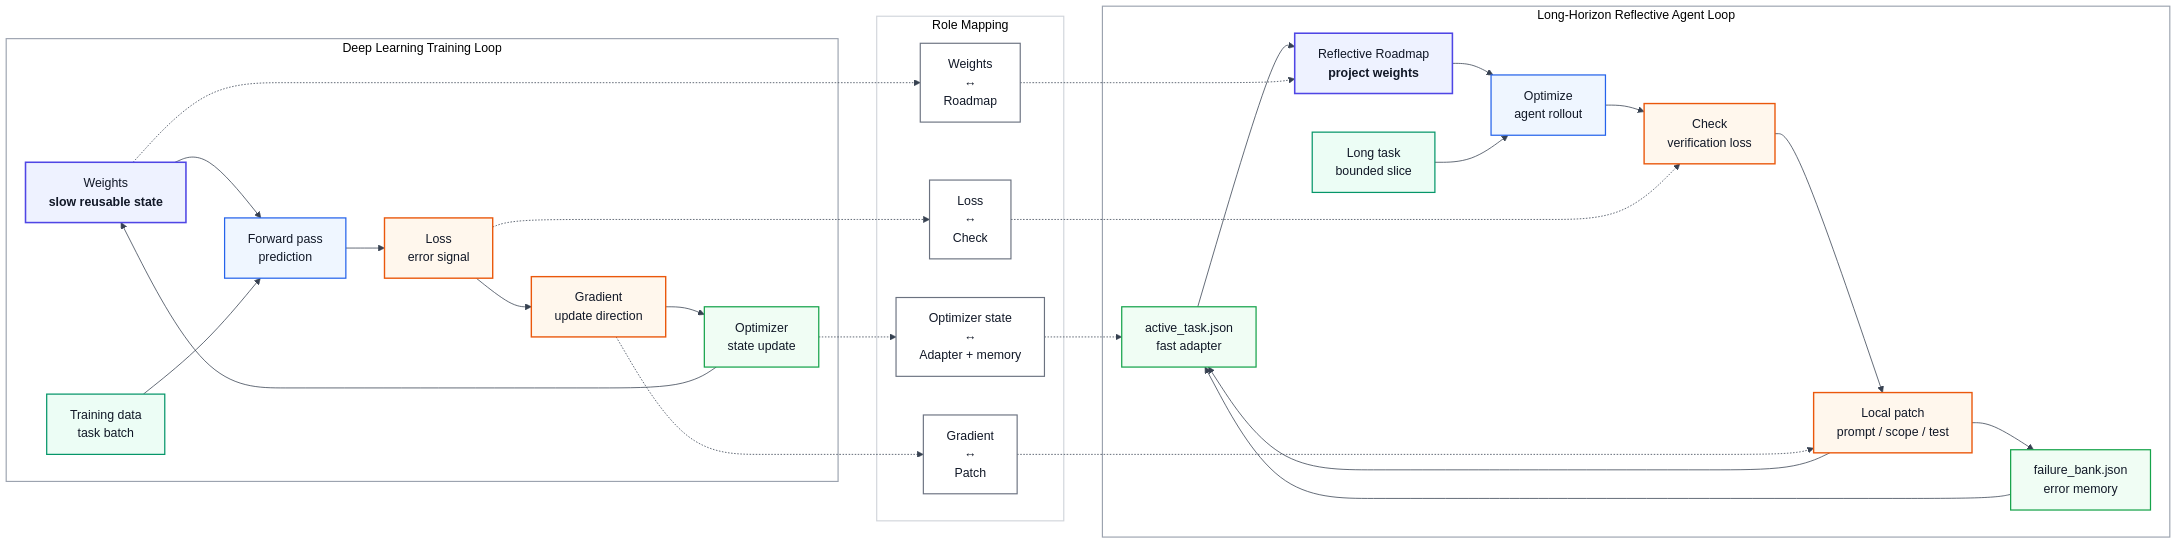
\includegraphics[width=\textwidth]{figures/training-view-agent-loop.png}
\caption{Training view of long-horizon agent loops. \ours{} does not update neural parameters; it imports the training structure into external state. The roadmap is the slow reusable state, while checks, patches, adapters, and failure memory implement a non-parametric update loop.}
\label{fig:overview}
\end{figure*}

Our framing is inspired by machine-learning optimization, but it is explicitly non-parametric. No base model weights are updated. Instead, the system updates external artifacts: roadmaps, task adapters, patches, logs, and failure banks. The analogy is not decorative; it explains why the roadmap matters. Just as pretrained weights carry reusable structure across downstream tasks, the roadmap carries project-level structure across agent epochs. Fast local state can adapt, but it should adapt against the stable backbone rather than rewriting the whole objective.

This paper makes three contributions. First, we formulate long-task coding loops through a roadmap-as-weights abstraction. Second, we describe a concrete seven-CLI implementation that keeps state, logs, and handoffs outside ephemeral chat context. Third, we show how the same abstraction scales to \texttt{moa-loop}: a mixture-of-agents computation graph with vertical serial epochs, horizontal DAG scheduling, and shared blackboard communication.

\section{Preliminaries and Problem Formulation}
\label{sec:definition}

\paragraph{Coding-agent episodes.}
Let $q$ denote a repository task and let an agent policy $\pi$ interact with a workspace through tool calls, shell commands, file edits, and tests. A one-shot agent produces a trajectory
\begin{equation}
\tau \sim \pi(\cdot \mid q),
\end{equation}
where $\tau$ contains observations, actions, tool outputs, and edits. For short tasks, a single trajectory may be enough. For long-horizon engineering, however, the desired object is not one trajectory but a sequence of recoverable epochs.

\begin{definition}[Reflective loop state]
A reflective loop state is a tuple
\begin{equation}
\mathcal{L}^{(k)} = \langle R, A^{(k)}, F^{(k)}, M^{(k)}, H^{(k)} \rangle,
\end{equation}
where $R$ is the roadmap, $A^{(k)}$ is the active task adapter, $F^{(k)}$ is the failure memory, $M^{(k)}$ records the current mode, and $H^{(k)}$ stores logs, snapshots, and handoff notes at epoch $k$.
\end{definition}

\paragraph{Slow and fast state.}
The roadmap $R$ stores durable project intent: goals, constraints, milestones, and non-negotiable design choices. It is analogous to a frozen or slowly updated backbone. The active adapter $A^{(k)}$ is a structured JSON record for the current slice of work. It stores local patches, immediate verification requirements, and the next bounded target. This separation prevents two common failures: global plans being overwritten by local errors, and local fixes being lost inside a long transcript.

\paragraph{Optimize/check epochs.}
Each epoch contains two conceptual phases. The optimize phase performs bounded implementation conditioned on $(R,A^{(k)},F^{(k)})$. The check phase reviews the result, estimates the residual error, and emits patch signals:
\begin{equation}
P^{(k)} = C(\tau^{(k)}, R, A^{(k)}, F^{(k)}),
\end{equation}
where $P^{(k)}$ may include prompt patches, scope patches, verification patches, and new failure patterns. The next state is updated externally:
\begin{equation}
A^{(k+1)}, F^{(k+1)}, H^{(k+1)} = U(A^{(k)}, F^{(k)}, H^{(k)}, P^{(k)}).
\end{equation}
This update is non-parametric: it changes files and structured state, not model weights.

\paragraph{Objective.}
Let $S(\tau,q)$ be a task success indicator and let $B(\tau)$ measure engineering cost, such as repeated failed attempts or redundant context reconstruction. \ours{} aims to improve long-horizon execution by increasing expected success while reducing repeated work:
\begin{equation}
\max_{\mathcal{L}} \; \mathbb{E}_{q}\left[S(\tau,q) - \lambda B(\tau)\right],
\end{equation}
subject to auditability: every epoch should leave enough state for a later agent or human to resume the project without relying on hidden context.


\section{\ours{} Design}
\label{sec:method}

\subsection{Long Tasks First}
\ours{} starts from a practical observation: the hard part of autonomous coding is not one patch, but continuity across many patches. A long task needs a stable objective, bounded local work, periodic checking, and a way to resume after the model, process, or human session stops. We therefore treat the loop as the primary unit of design. The CLI call is only one forward pass inside a larger training-like procedure.

\subsection{Unified Loop Skill Interface}
\ours{} packages the same long-task loop abstraction for seven agent CLIs plus one multi-agent orchestrator. Each skill directory contains a human-readable \texttt{SKILL.md}, a default prompt, an initialization script, a daemon runner, and state files. The CLI-specific layer handles dispatch and model invocation; the loop semantics remain shared. This design makes the loop portable: Codex, Gemini, Claude, Qwen, Kimi, MiniMax, and Cursor can use different command interfaces while preserving the same state machine.

\begin{table*}[t]
\centering
\small
\resizebox{\textwidth}{!}{%
\begin{tabular}{lllll}
\toprule
Skill & CLI target & State directory & Initializer & Core persistent state \\
\midrule
\texttt{codex-loop} & \texttt{codex} & \texttt{.codex-loop/state} & \texttt{init\_codex\_loop.cjs} & roadmap, \activestate{}, \failurebank{}, \lastmode{} \\
\texttt{gemini-loop} & \texttt{gemini} & \texttt{.gemini-loop/state} & \texttt{init\_gemini\_loop.cjs} & roadmap, \activestate{}, \failurebank{}, \lastmode{} \\
\texttt{claude-loop} & \texttt{claude} & \texttt{.claude-loop/state} & \texttt{init\_claude\_loop.cjs} & roadmap, \activestate{}, \failurebank{}, \lastmode{} \\
\texttt{qwen-loop} & \texttt{qwen} & \texttt{.qwen-loop/state} & \texttt{init\_qwen\_loop.cjs} & roadmap, \activestate{}, \failurebank{}, \lastmode{} \\
\texttt{kimi-loop} & \texttt{kimi} & \texttt{.kimi-loop/state} & \texttt{init\_kimi\_loop.cjs} & roadmap, \activestate{}, \failurebank{}, \lastmode{} \\
\texttt{minimax-loop} & \texttt{mmx} & \texttt{.minimax-loop/state} & \texttt{init\_minimax\_loop.cjs} & roadmap, \activestate{}, \failurebank{}, \lastmode{} \\
\texttt{cursor-loop} & \texttt{cursor} & \texttt{.cursor-loop/state} & \texttt{init\_cursor\_loop.cjs} & roadmap, \activestate{}, \failurebank{}, \lastmode{} \\
\texttt{moa-loop} & multi-agent & \texttt{.moa-loop/state} & \texttt{init\_moa\_loop.cjs} & roadmap, blackboard, DAG, iterations \\
\bottomrule
\end{tabular}}
\caption{The eight loop skills share the same persistent state abstraction while adapting to different agent CLIs. \texttt{moa-loop} extends the interface with DAG scheduling and shared blackboard.}
\label{tab:skills}
\end{table*}

\subsection{Roadmaps as Weights}

The central design choice is to make the deep-learning metaphor operational. \Cref{tab:mapping} summarizes the mapping. The roadmap is not a prompt fragment; it is the durable backbone of the project. In practice, we found that roadmap quality dominates long-task stability in the same way that pretrained weights dominate downstream adaptation. \activestate{} is not a log; it is the fast local adapter that captures the current slice. The check phase is not merely a reviewer; it computes backward signals that update the next optimize phase. \failurebank{} is not a transcript archive; it is an abstracted memory of error patterns and mitigations.

\begin{table}[t]
\centering
\small
\resizebox{\columnwidth}{!}{%
\begin{tabular}{ll}
\toprule
ML concept & \ours{} component \\
\midrule
Pretrained backbone & Roadmap / global plan \\
PEFT or LoRA adapter & \activestate{} local state \\
Forward pass & Optimize phase \\
Loss signal & Check phase findings \\
Backpropagation signal & Local patches \\
Training epoch & One optimize/check cycle \\
Checkpoint & Snapshot and handoff logs \\
Catastrophic forgetting control & \failurebank{} \\
\bottomrule
\end{tabular}}
\caption{The deep-learning analogy used by \ours{} is non-parametric: all updates are external state updates.}
\label{tab:mapping}
\end{table}

\subsection{Vertical Iteration}

The vertical loop is intentionally serial. At epoch $k$, the agent reads the roadmap, failure bank, and active adapter; performs one bounded optimize pass; runs or records verification; then enters a check pass. The check pass writes structured local patches and updates failure memory. Epoch $k+1$ begins only after the previous state has been persisted. This ordering trades some latency for correctness: project state remains traceable, interruptions are recoverable, and a later agent can inspect why a decision was made.

\begin{algorithm}[t]
\caption{\ours{} vertical epoch}
\label{alg:epoch}
\begin{algorithmic}[1]
\STATE Read roadmap $R$, adapter $A^{(k)}$, and failure bank $F^{(k)}$
\STATE Select one bounded target from $A^{(k)}$
\STATE Run optimize pass and record trajectory $\tau^{(k)}$
\STATE Run check pass against $R$, target, and verification evidence
\STATE Emit local patches $P^{(k)}$
\STATE Persist updated adapter, failure bank, mode, logs, and handoff
\end{algorithmic}
\end{algorithm}

\subsection{Loop Trigger Boundaries}

Different systems implement ``loop'' at different trigger boundaries. Claude/Ralph-style loops intercept the runtime stop point: a Stop hook can return a blocking decision and refeed a reason into the next model step. Codex-style loops use external time: a shell or Python daemon sleeps, wakes, and resumes the same thread through \texttt{codex exec resume}. LikeCode-style \texttt{/loop} behaves like cron at the user level, but it is not Linux \texttt{crontab}; it is an application-level scheduler that creates tasks and later enqueues prompts inside the running app. \ours{} abstracts over these mechanisms by requiring every trigger to produce the same epoch contract: read roadmap, run a bounded slice, check, persist patches, and prepare the next epoch.

\begin{table*}[t]
\centering
\small
\resizebox{\textwidth}{!}{%
\begin{tabular}{llll}
\toprule
Mechanism & Trigger boundary & Continuation method & State implication \\
\midrule
Claude/Ralph Hook & Runtime \texttt{Stop} event & Block stop and refeed reason & Strong lifecycle control, runtime-specific \\
Codex external daemon & External \texttt{while}/sleep tick & Resume same thread with prompt & Portable, process-managed state and logs \\
LikeCode \texttt{/loop} & Application-level cron scheduler & Enqueue scheduled prompt & User-friendly task registry, app-managed timing \\
OS-level cron & System scheduler (\texttt{crontab}) & Health-check and restart daemon & Machine-level supervision, reboots, crash recovery \\
\ours{} contract & Persistent epoch boundary & Optimize/check with roadmap state & Trigger-agnostic long-task optimization \\
\bottomrule
\end{tabular}}
\caption{Loop mechanisms differ in where they trigger continuation. \ours{} focuses on the state contract that should survive any trigger boundary.}
\label{tab:loop_triggers}
\end{table*}

\subsection{\texttt{moa-loop}: From One Loop to a Computation Graph}

The repository also includes \texttt{moa-loop}, and it should be part of the paper because it answers the scaling question: what happens after a single long-task loop becomes multiple cooperating agents? We treat \texttt{moa-loop} as the multi-agent generalization of \ours{}, not as an eighth CLI wrapper. In this view, the roadmap remains the frozen backbone, subtask adapters act like PEFT-style local updates, the optimize/check cycle remains the training epoch, and the DAG becomes the computation graph.

Concretely, independent nodes such as research, documentation, and tests may run in parallel, while dependent nodes remain serial. A centralized shared blackboard stores horizontal working state, avoiding point-to-point message storms. The key rule is separation of concerns: horizontal coordination optimizes latency inside an epoch, while vertical persistence preserves ordered project evolution across epochs. Thus \texttt{moa-loop} is the bridge from persistent single-agent loops to mixture-of-agents training dynamics.

\subsection{Two-Layer Communication}

The communication design follows the reference architecture in \texttt{references/ref1.txt}. Horizontal communication favors a shared blackboard for low-latency multi-agent coordination. Vertical communication favors structured persistence: Markdown for human-readable intent, JSON for compact active state, and SQL or file-backed logs for durable indexing and replay. The two layers should not replace each other. Shared memory is fast but ephemeral; persistent JSON and logs are slower but auditable and resumable.

\subsection{Daemon Management and Health Supervision}

Every loop skill ships a unified daemon management interface. Four scripts---\texttt{start}, \texttt{stop}, \texttt{status}, and \texttt{print\_cron\_entry}---provide OS-level process supervision independent of the agent CLI. The start script launches the daemon in a detached tmux session or nohup background process, writes a PID file for health checks, and refuses to start a second instance. The stop script sends SIGTERM, waits for graceful shutdown, and falls back to SIGKILL if the process does not exit within five seconds. The status script reads the PID file, checks whether the process is alive, and reports the current mode plus recent log activity.

The \texttt{print\_cron\_entry} script generates ready-to-use crontab entries: an \texttt{@reboot} rule for auto-starting after machine restart, and a periodic health-check rule that runs the status script and triggers a restart on failure. Each skill uses a health-check interval tuned to its workload characteristics, summarized in \cref{tab:cron}.

\begin{table}[t]
\centering
\small
\resizebox{\columnwidth}{!}{%
\begin{tabular}{lcl}
\toprule
Skill & Interval & Rationale \\
\midrule
\texttt{gemini-loop} & \texttt{*/5}  & Fast iteration, reference agent \\
\texttt{codex-loop}  & \texttt{*/10} & Balanced, production-stable \\
\texttt{claude-loop} & \texttt{*/10} & Production-grade stability \\
\texttt{cursor-loop} & \texttt{*/15} & IDE integration, lower frequency \\
\texttt{kimi-loop}   & \texttt{*/15} & Long-context tasks, wider interval \\
\texttt{minimax-loop}& \texttt{*/5}  & Lightweight, fast patrol \\
\texttt{qwen-loop}   & \texttt{*/10} & Balanced strategy \\
\texttt{moa-loop}    & \texttt{*/5}  & Multi-agent, frequent checks \\
\bottomrule
\end{tabular}}
\caption{Differential cron health-check intervals. Faster intervals target lightweight or multi-agent skills; slower intervals suit IDE-integrated or long-context skills.}
\label{tab:cron}
\end{table}

This separation of concerns means that the loop optimization logic inside each skill remains independent of how the process is supervised. A developer can run the daemon manually, under tmux, via cron, or under systemd, and the epoch contract remains the same.

\section{Lightweight Validation}
\label{sec:experiment}

This paper does not claim benchmark-scale empirical improvements. Instead, we validate whether the repository realizes the proposed long-task abstraction and whether the artifacts support the intended roadmap-to-adapter-to-patch workflow.

\paragraph{Structural validation.}
We inspect the eight skill directories and verify that each exposes the same interface family: \texttt{SKILL.md}, an initializer, a daemon runner, daemon management scripts, and persistent state files. \Cref{tab:skills} shows the resulting comparison. The shared structure supports the main portability claim: loop semantics are independent of the underlying CLI target.

\paragraph{Roadmap-to-patch case.}
A typical epoch starts from the roadmap and selects a bounded task in \activestate{}. The optimize phase attempts the task and records evidence. If verification fails, the check phase should not simply report failure. It should produce a localized patch, for example: a prompt patch that changes how the agent reasons, a scope patch that narrows the edit radius, or a verification patch that adds a missing test. The next optimize phase consumes the patch while still being constrained by the roadmap backbone. This makes the failure reusable across epochs without requiring the next agent to reread the entire transcript.

\begin{table}[t]
\centering
\small
\resizebox{\columnwidth}{!}{%
\begin{tabular}{lll}
\toprule
Removed component & Expected degradation & Observable symptom \\
\midrule
Roadmap & Plan drift & Local fixes violate global goals \\
\activestate{} & Weak adaptation & Next epoch repeats setup work \\
\failurebank{} & Forgetting & Recurring errors reappear \\
Check phase & No backward signal & Failures become pass/fail notes \\
Logs/snapshots & Poor auditability & Resume depends on chat context \\
DAG scheduler & Low parallelism & Independent work is serialized \\
Cron health check & No crash recovery & Daemon stays dead after failure \\
\bottomrule
\end{tabular}}
\caption{Lightweight ablation analysis of the reflective loop design.}
\label{tab:ablation}
\end{table}

\paragraph{Design-level ablation.}
\Cref{tab:ablation} summarizes expected degradations when individual components are removed. These are not presented as measured benchmark results; they are acceptance criteria for the architecture. For example, if removing \failurebank{} does not make repeated failures harder to prevent, then the memory abstraction is not carrying useful information. If removing the check phase does not change future behavior, then the loop is only logging rather than optimizing.

\paragraph{Takeaway.}
The repository satisfies the core implementation requirements for long-task loop optimization: shared loop structure across CLIs, explicit roadmap/adapter state separation, auditable mode transitions, and an extension path from single-agent vertical epochs to multi-agent DAG coordination.

\section{Related Work}

\paragraph{LLM agents and coding agents.}
Recent LLM agents use tools, executable actions, and environment feedback to solve increasingly complex tasks \citep{codeact,alphaevolve,automind}. These systems demonstrate that agentic execution can outperform static prompting when tasks require interaction and revision. \ours{} is complementary: it does not propose a new base policy, but a persistence layer that helps coding agents continue work across repeated sessions and checks.

\paragraph{Experience learning and agent memory.}
Prior work studies experiential learning, workflow memory, procedural memory, and agentic memory \citep{expel,awm,memp,legomem,xu2025amemagenticmemoryllm,reme}. These methods store reusable knowledge from prior trajectories. \ours{} shares the goal of reuse, but targets repository-level engineering state rather than only task-level behavior. Its memory is split into roadmap, active adapter, logs, and failure bank so that different temporal scales can evolve independently.

\paragraph{Skills and reusable procedures.}
Skill libraries provide reusable abstractions for agent behavior, ranging from embodied skills to tool-use procedures \citep{voyager,anthropic_skills}. \ours{} treats each loop skill as a reusable orchestration skill: it teaches a CLI agent how to plan, optimize, check, and persist state. The focus is therefore not a domain skill such as web navigation, but a meta-skill for sustained engineering.

\paragraph{Multi-agent orchestration.}
Multi-agent systems often require dependency-aware scheduling and shared communication substrates. The horizontal DAG extension in \ours{} follows this direction by separating parallelizable subtasks from causally dependent ones. The vertical loop ensures that such parallelism does not erase temporal order: every epoch still produces a recoverable state transition.

\paragraph{Loop mechanisms in agent runtimes.}
Existing agent products expose different continuation mechanisms. Hook-based systems can intercept lifecycle events such as stopping; daemon-based systems can resume an external process on a timer; and application-level cron systems can schedule prompts inside the app event loop. These mechanisms differ operationally, but they share the same research question for long tasks: what state must persist between invocations? \ours{} argues that the roadmap, adapter, patches, and failure bank are the minimum state needed to make those invocations behave like optimization rather than repetition.

\section{Conclusion}

We presented \systemname{}, a systems pattern for turning long-horizon coding-agent work into persistent, auditable optimization loops. The core lesson is simple: for long tasks, roadmaps are weights. They carry the slow project knowledge that local adapters and patches should update against, not overwrite. Across seven CLI-specific skills and one multi-agent orchestrator, \ours{} uses the same non-parametric deep-learning analogy: roadmaps act as slow backbones, active task files act as fast adapters, check phases produce backward signals, local patches guide the next optimize pass, and failure banks preserve reusable error memory. We further described hook, daemon, OS-level cron, and application-level loop boundaries, and included \texttt{moa-loop} as the natural extension from one persistent loop to a mixture-of-agents computation graph.

The immediate value of \ours{} is practical: it gives coding agents a concrete way to continue long-running work without relying on hidden chat context. Future work should add benchmark-scale evaluation, stronger state schemas, richer visual monitoring, and adapters for hosted agent runtimes where file-system persistence is not available by default.


\section*{Impact Statement}
This work aims to make long-running coding agents more transparent, reproducible, and recoverable. Persistent roadmaps and failure memories may reduce repeated computation and make agentic engineering easier to audit. The same persistence can also preserve stale assumptions or unsafe behaviors if the check phase is weak; therefore, \ours{} treats the roadmap and failure memory as inspected artifacts rather than hidden model state.

\section*{Limitations}
\ours{} is a systems pattern and repository implementation, not a trained model. The present paper reports lightweight structural validation rather than benchmark-scale task success rates. The phrase ``roadmaps as weights'' is a conceptual analogy for non-parametric state updates; it should not be read as gradient training of neural parameters. The current implementation also assumes file-system persistence and CLI agents, so hosted or stateless agent runtimes require adapters.

\bibliography{references}
\bibliographystyle{icml2026}

\newpage
\appendix
\onecolumn
\section{Appendix}

\subsection{Repository Layout}

Each primary loop skill follows the same layout:
\begin{verbatim}
<name>-loop/
  README.md
  SKILL.md
  prompt.md
  scripts/
    init_<name>_loop.cjs
    run_daemon.py
    run_daemon.sh
    start_<name>_loop.sh
    stop_<name>_loop.sh
    status_<name>_loop.sh
    print_cron_entry.sh
\end{verbatim}

\subsection{Example Active Task Schema}

\begin{verbatim}
{
  "plan_id": "PROJECT_ROADMAP",
  "mode": "optimize",
  "bounded_target": "complete one verifiable slice",
  "prompt_patch": [],
  "scope_patch": [],
  "verification_patch": [],
  "handoff": "next smallest useful action"
}
\end{verbatim}

\subsection{Example Failure Memory Entry}

\begin{verbatim}
{
  "failure_type": "verification_gap",
  "symptom": "implementation completed without running target tests",
  "patch": "before final handoff, run the smallest relevant check",
  "seen_in": ["epoch-004", "epoch-009"]
}
\end{verbatim}

\subsection{Daemon Management Commands}

All loop skills share the same management interface:

\begin{verbatim}
# Initialize state
node <skill>-loop/scripts/init_<name>_loop.cjs MY_ROADMAP

# Start daemon (tmux/nohup auto-select)
bash <skill>-loop/scripts/start_<name>_loop.sh MY_ROADMAP

# Check status (PID health + last mode)
bash <skill>-loop/scripts/status_<name>_loop.sh MY_ROADMAP

# Stop daemon gracefully (SIGTERM -> SIGKILL)
bash <skill>-loop/scripts/stop_<name>_loop.sh MY_ROADMAP

# Print cron entries for OS-level supervision
bash <skill>-loop/scripts/print_cron_entry.sh
\end{verbatim}

\subsection{Cron Integration Example}

The following crontab entries provide automatic restart after reboot and periodic health checks:
\begin{verbatim}
# Auto-start after reboot
@reboot cd /workspace && <SKILL>_LOOP_WORKSPACE=/workspace \
  bash /path/to/start_<name>_loop.sh

# Health check every N minutes (restart on failure)
*/N * * * * cd /workspace && \
  bash /path/to/status_<name>_loop.sh \
  || bash /path/to/start_<name>_loop.sh
\end{verbatim}

\subsection{Implementation Notes}

The Codex and MOA loops include additional monitoring commands:
\begin{verbatim}
# Codex: real-time monitoring dashboard
bash codex-loop/scripts/monitor_codex_loop.sh --watch

# MOA: DAG + Blackboard + PEFT dashboard
bash moa-loop/scripts/monitor_moa_loop.sh --watch
\end{verbatim}

The MOA loop extends the abstraction with \texttt{dag\_scheduler.py}, \texttt{shared\_blackboard.py}, and \texttt{iteration\_manager.py}. These modules implement horizontal DAG scheduling, centralized agent communication, and epoch-level PEFT adaptation tracking.


\end{document}
